\documentclass[border = .2cm]{standalone}
\usepackage{tikz}
\usepackage{tkz-graph}
\usepackage{amsmath,amssymb}
\usepackage{xcolor}
\usetikzlibrary{calc}
\usetikzlibrary{positioning}

\usepackage{pgfplots}
\pgfplotsset{compat=newest}

% https://latexdraw.com/three-dimensional-plotting-in-latex/
\begin{document}


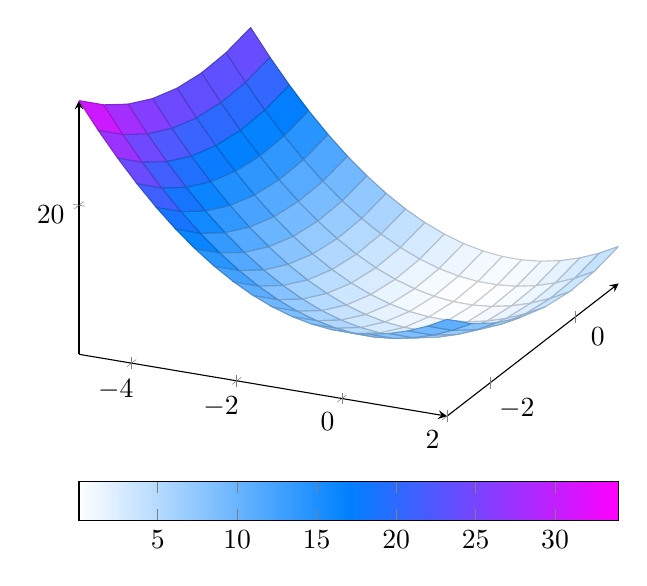
\begin{tikzpicture}
	\begin{axis}[colormap/cool, colorbar horizontal, axis lines  = left]
		\addplot3 [
			domain=-5:2,
			domain y = -3:1,
			samples = 20,
			samples y = 8,
			surf,
		] {x^2 + y^2};
	\end{axis}
\end{tikzpicture}


\end{document}


